
\begin{frame}[fragile]{Length}{absolute values}\relax
    \def\showLength#1{\raise4pt\hbox{\vrule height 6pt depth2pt{\csk\rule{#1}{4pt}}\vrule height 6pt depth2pt} #1}
    
    \centering
    most common used:
    
    \begin{tabular}{r|cc|l}
         pt& points & $\simeq$0.35mm & \showLength{12pt} \\
         mm& millimeters & $\simeq$2.84pt & \showLength{10mm} \\
         cm& centimeter & $\simeq$28.4pt, 10mm & \showLength{1cm} \\
         in& inch & $\simeq$72.27pt, $\simeq$, 25.4mm  & \showLength{1in} \\
    \end{tabular}
    
    
    \skfootnote{\wikiC{https://en.wikibooks.org/wiki/LaTeX/Lengths} \knuthc{10}[68] \lvoc{I.2.10}[26]}
\end{frame}


\begin{frame}[fragile]{Length}{absolute values\magicPage}\relax
    \def\showLength#1{\raise4pt\hbox{\vrule height 6pt depth2pt{\csk\rule{#1}{4pt}}\vrule height 6pt depth2pt} #1}
    
    \centering
    not so common used:
    
    \begin{tabular}{r|cc|l}
         pt& points & $\simeq$0.35mm & \showLength{12pt} \\
         mm& millimeters & $\simeq$2.84pt & \showLength{10mm} \\\hline
         bp& big point & 1/72in, $\simeq$1.003pt & \showLength{12bp} \\
         pc& pica & 12pt, 4.2mm  & \showLength{1pc} \\
         dd& didot & $\simeq$1.07pt, $\simeq$0376mm  & \showLength{12dd} \\
         cc & cicero & 12dd & \showLength{1cc}\\ \hline
         sp & scaled point    & 1/$2^{16}$pt = 1/65536pt & \showLength{2097152sp} \\
    \end{tabular}
    
    (pt and mm here for comparison)
    
    \inclasshigh{The \textbf{sp} seems to be more ``programming'', not ``typography'' unit, isn't it?} 
    
    Every \TeX's length is a integer number of {\csk sp}
    
    \skfootnote{\wikiC{https://en.wikibooks.org/wiki/LaTeX/Lengths} \knuthc{10}[68] \lvoc{I.2.10}[26]}
\end{frame}

\begin{frame}[fragile]{Length}{Relative values}\relax
    \def\showLength#1{\raise4pt\hbox{\vrule height 6pt depth2pt{\csk\rule{#1}{4pt}}\vrule height 6pt depth2pt} #1}
    
    \centering
    
    
    \begin{tabular}{r|c|l}
         pt& points  & \showLength{12pt} \\
         mm& millimeters & \showLength{10mm} \\\hline
         em& roughly the {\csk width} of an {\csk 'M'} (uppercase) & \showLength{1em} \\
         ex& roughly the {\csk height} of an {\csk 'x'} & \showLength{1ex} \\\hline
    \end{tabular}
    
    \inpause example: \verb|\Huge|
    
    \begin{tabular}{r|l}
         mm & \showLength{10mm} \\
         em & \showLength{1em} \\\hline
         \Huge mm & \Huge \showLength{10mm} \\
         \Huge em & \Huge \showLength{1em} \\
    \end{tabular}
    
    use {\csk em} for horizontal and {\csk ex} for vertical cases
    
    \skfootnote{\wikiC{https://en.wikibooks.org/wiki/LaTeX/Lengths} \knuthc{10}[68] \lvoc{I.2.10}[26]}
\end{frame}

\begin{frame}[fragile]{Prebuild lengths}{Most used}\relax

    \centering
    \begin{tabular}{r|l}
        \multicolumn{2}{c}{\tiny\TeX's}\\\hline
         \ccol\parindent & The normal paragraph indentation\\
         \ccol\parskip & The extra vertical space between paragraphs \\
         \hline\multicolumn{2}{c}{\tiny\LaTeX's}\\\hline
         \ccol\textwidth & The width of the text on the page\\
         \ccol\textheight & The height of the text on the page\\
         \ccol\linewidth & The width of the text in this ``box''\\
         \ccol\lineheight & The height of the text in this ``box''\\
    \end{tabular}
    
     By typography rules, don't put both parskip and parindent as paragraph separation.

     \skfootnote{\wikiC{https://en.wikibooks.org/wiki/LaTeX/Lengths\#LaTeX_default_lengths} \lmanc{5.5}[34] \stExC{https://tex.stackexchange.com/questions/16942/difference-between-textwidth-linewidth-and-hsize}\\ 
     \ccol\parskip\ is actually a glue.  You can define your own lengths (See next lecture.)}
\end{frame}

\begin{frame}[fragile]{Prebuild lengths\magicPage}{not so common used}
     \centering {\LaTeX}\par
     practicully every length --- the margins; footnote, footer/header place; distance between columns,..\\[2ex]
     \TeX\par
     \begin{tabular}{rl}
    \ccol\hsize, \ccol\vsize & the normal size of text in page \\
    \ccol\hoffset, \ccol\voffset & the offset of on page 
     \end{tabular}
     
     
     \skfootnote{\lvoc{IV.4}[166] \lmanc{5.5}[34]\\ 
     by the way, you can magnitude whole text by \ccol\mag=... parameter.
     Also there are \ccol\hangindent\ and \ccol\hangafter\ \TeX\ params, but we'll speak in paragraph section. 
     }
\end{frame}

\begin{frame}\relax\magicPage
    \centering
    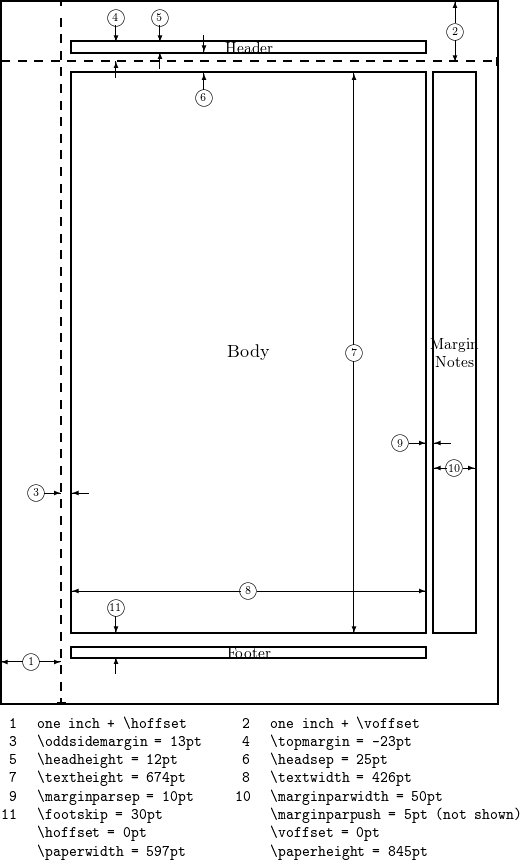
\includegraphics[height=0.9\textheight]{Layout-dimensions}
         
    \skfootnote{\overC{https://www.overleaf.com/learn/latex/Page_size_and_margins}}
\end{frame}

\begin{frame}[fragile, t]{How to use lengths}\relax

    \inclassFrag{
    compile a document with different \ccol\parindent\ lengths
    % \lstinputlisting{lengthsTASK.tex}
    \inputminted[firstline=6, lastline=8]{latex}{sec/code/lengthsTASK.tex}
    }[1]
    
    \samePosPictureI{sec/code}{lengthsAr1}{11-11,18-20}
   

    Just \ccol{\<length-command>=<length>}

\end{frame}


\begin{frame}[fragile,t]{How to use lengths}\relax

    \samePosPictureI{sec/code}{lengthsAr2}{11-11,18-21}
    
    Arifmetics: {\csk <multiply-factor>\ccol\<length-command>}

\end{frame}

\begin{frame}[fragile,t]{How to use lengths}\relax

    \samePosPictureI{sec/code}{lengthsAr3}{11-11,18-22}
    
    Arifmetics: BUT You can't use simple notation {\csk +, -, /, *,...}
     % lengthsAr 18-20, 21-21, 22-22, 23-24
\end{frame}

\begin{frame}[fragile,t]{How to use lengths}\relax

    \samePosPictureI{sec/code}{lengthsAr4}{11-11,18-24}
    
    Arifmetics: \ccol{\dimexpr} allow to use ``normal'' notation. 
    
    \skfootnote{\stExC{https://tex.stackexchange.com/questions/245635/formal-syntax-rules-of-dimexpr-numexpr-glueexpr}}
\end{frame}

%%%%%%%%%%%%% manipulation %%%%%%%%%%%%
\begin{frame}{Length manipulation\lW}\relax

    \textbf{Define length} \ccol{\newlength\{\string\<lenname>\}}
    
    \textbf{Set length} \ccol{\setlength}
    
    \textbf{Add length}  \ccol{\addtolength}. 
    
    \textbf{Show length} \ccol{\the\string\<lenname>}. But also you can use \ncol\usepackage{printlen}\ and then \ccol\uselengthunit, \ccol\printlength
    
    
    
    \skfootnote{\wikiC{https://en.wikibooks.org/wiki/LaTeX/Lengths} }
\end{frame}

\begin{frame}{Length manipulation\lW}{Example}\relax

    \twocolImg{
    % \lstinputlisting[linerange={7-7,11-16}]{lengthLaTeX.tex}
    \inputminted[firstline=7, lastline=7]{latex}{sec/code/lengthLaTeX.tex}
    \inputminted[firstline=11, lastline=16]{latex}{sec/code/lengthLaTeX.tex}
    }{lengthLaTeX.pdf}


\end{frame}



\begin{frame}[fragile]{Length manipulation\tW}\relax

    \textbf{Define length} \ccol{\newdimen\string\<lenname>}
    
    \textbf{Set length} \ccol{\<lenname>=<len>}
    
    \textbf{Add length}  \ccol{\advance \string\<lenname>\ by <len>}. Also there are \ccol\multiply\ and \ccol\divide. As well as \ccol\dimexp.
    
    \textbf{Show length} \ccol{\the \\<lenname>}
    
    % \textbf{Compare lengths} \ccol\ifdim\\firstLen>\\secondLen 
    
    
    \skfootnote{\knuthc{15}[132] }
\end{frame}

\begin{frame}{Length manipulation\tW}{Example}\relax

    \twocolImg{
    % \lstinputlisting[linerange={11-14}]{lengthTeX.tex}
        \inputminted[firstline=11, lastline=14]{latex}{sec/code/lengthTeX.tex}
    }{lengthTeX.pdf}

\end{frame}



